%Based on the code of Yiannis Lazarides
%http://tex.stackexchange.com/questions/42602/software-requirements-specification-with-latex
%http://tex.stackexchange.com/users/963/yiannis-lazarides
%Also based on the template of Karl E. Wiegers
%http://www.se.rit.edu/~emad/teaching/slides/srs_template_sep14.pdf
%http://karlwiegers.com
\documentclass{scrreprt}
\usepackage{listings}
\usepackage{underscore}
\usepackage[margin=3.0cm]{geometry}
\usepackage{enumitem}
\usepackage{graphicx,subfigure}
\usepackage[bookmarks=true]{hyperref}
\usepackage[english, spanish]{babel}
\usepackage[utf8]{inputenc}
\usepackage{float}
\usepackage{xcolor}
\usepackage{fancyhdr}
\usepackage[export]{adjustbox}
\usepackage{tabularx}

\hypersetup{
    bookmarks=false,        % show bookmarks bar?
    pdftitle={Especificación de Requerimientos de Software},    % title
    pdfauthor={},           % author
    pdfsubject={},          % subject of the document
    pdfkeywords={},         % list of keywords
    colorlinks=true,        % false: boxed links; true: colored links
    linkcolor=blue,         % color of internal links
    citecolor=black,        % color of links to bibliography
    filecolor=black,        % color of file links
    urlcolor=purple,        % color of external links
    linktoc=page            % only page is linked
}

\def\myversion{1.0}
\date{}
\usepackage{hyperref}
\usepackage{etoolbox}

%%%%%%%%%%%
% Configurar estilo de header y footer
\fancypagestyle{plain}{
  \fancyhf{}
  \lfoot{
\includegraphics[scale=0.08,valign=c]{images/space_logo.png}}
  \rfoot{Pág. \thepage}
}

\pagestyle{fancy}
\fancyhf{}
\lfoot{
\includegraphics[scale=0.08,valign=c]{images/space_logo.png}}
\rfoot{Pág. \thepage}

\renewcommand{\headrulewidth}{0pt} % linea de header invisible
\renewcommand{\footrulewidth}{0.4pt} % linea de footer delgada

%%%%%%%%%%

\begin{document}

\begin{flushright}
	\rule{16cm}{0.2cm}\vskip1cm
    \begin{bfseries}
        \Huge{DOCUMENTO DEL \\ AVANCE \#2}\\
        \vspace{0.5cm}
        para\\
        \vspace{0.5cm}
        Sistema de preprocesamiento y segmentación de células\\
        \vspace{1.0cm}
        \LARGE{Versión \myversion}\\
        \vspace{1.0cm}
        Preparado por:\\ \vspace{0.5cm}
        	José Alvarado Chaves, 201129079\\
            Reggie Barker Guillén, 2014050578\\
            Joel Barrantes Garro, 2013120962\\
            Joel Schuster Valverde, 2014096796\\                        
        \vspace{1.5cm}
        Instituto Tecnológico de Costa Rica\\
        \vspace{1.5cm}
        \today\\
    \end{bfseries}
\end{flushright}


\tableofcontents



%%%%%%%%%%%%%%%%%%%%%%%%%%%%%%%%%%%%%%%%%%%%%%%%%%%%%%%%%
%%% Link al documento estandar ISO-IEC-IEEE 29148-2011 %%
%%% http://docdro.id/LvmnK4Y					       %%	 
%%%%%%%%%%%%%%%%%%%%%%%%%%%%%%%%%%%%%%%%%%%%%%%%%%%%%%%%%

\chapter{Unidades de diseño}

En este capitulo, se relacionan los ítems de diseño identificados anteriormente con los requerimientos y los artefactos de la arquitectura.

\section{Validación del sistema}

En la siguiente tabla se muestra cada item de diseño asociado y su correspondencia con los requerimientos descritos en la Especificación de Requerimientos del Sistema(SyRS):

\begin{center}
    \begin{tabular}{|p{1.5cm}|p{5.0cm}|p{7.5cm}|}
        \hline
	    Número de item & Nombre de item & Requerimiento asociado \\
        \hline
	    1 & Diagrama de clases del sistema.  & Procesamiento de lotes de imágenes en el sistema;  \\
        \hline        
        2 & Diagrama de estados de procesamiento de un lote.  &  Subida de imágenes; Procesamiento de lotes de imágenes en el sistema; Notificación de procesamiento del lote  \\
        \hline
        3 & Diagrama de componentes del sistema. &  Pre-procesamiento de lotes de imágenes en el sistema; \\
        \hline
        4 & Diagrama de despliegue del sistema. & Subida de imágenes; Descarga de imágenes procesadas del lote\\
        \hline
        5 & Diagrama de actividad de la interacción entre usuario y sistema. & Manejo de sesiones de usuario;  Visualización de lotes pendientes;  Descarga de imágenes procesadas del lote; Notificación de procesamiento del lote\\
        \hline
        6 & Diagrama de casos de uso del investigador. &  Visualización de lotes pendientes;  Descarga de imágenes procesadas del lote; Informe de resultados del procesamiento de un lote \\
        \hline
        7 & Diagrama de Entidad-Relación. & Manejo de sesiones de usuario; \\
        \hline
        8 & Diagrama de mongoDB & Subida de imágenes;  Descarga de imágenes procesadas del lote;\\
        \hline
        
    \end{tabular}
\end{center}

\section{Validación de la implementación}

La siguiente tabla muestra relación entre los items de implementación con los items de diseño del sistema:


\begin{center}
    \begin{tabular}{|p{1.5cm}|p{5.0cm}|p{7.5cm}|}
        \hline
	    Número de item & Nombre de item & Item de implementación \\
        \hline
	    1 & Diagrama de clases del sistema.  & Clases del \textit{package} tec.psa;  \\
        \hline        
        2 & Diagrama de estados de procesamiento de un lote.  & Imagen.java; Lote.java  \\
        \hline
        3 & Diagrama de componentes del sistema. & Spring Framework;  \\
        \hline
        4 & Diagrama de despliegue del sistema. & Spring Framework; \\
        \hline
        5 & Diagrama de actividad de la interacción entre usuario y sistema. & Spring MVC;  dashboard.html; login.html; registration.html; upload.html\\
        \hline
        6 & Diagrama de casos de uso del investigador. &Spring MVC;  dashboard.html; login.html; registration.html; upload.html\\
        \hline
        7 & Diagrama de Entidad-Relación. &  Clases del \textit{package} tec.psa.model; tablas.sql \\
        \hline
        8 & Diagrama de mongoDB & ImageManagement.java; mongoScript.bson \\
        \hline
        
    \end{tabular}
\end{center}

\chapter{Estándares}

\subsection{Estándar de codificación}

Durante el desarrollo del sistema SPACE, el equipo seguirá el estándar de codificación de Google, conocido como el \textit{Google Java Style} para la codificación en el lenguaje de programación \textit{Java}. Este estándar, junto al de Sun, es uno de los más populares entre los desarrolladores de Java, y sus lineamientos actualizados pueden encontrarse fácilmente en la web: \href{https://google.github.io/styleguide/javaguide.html}{https://google.github.io/styleguide/javaguide.html}\\

Entre las razones para favorecer a este estándar de codificación, están

\begin{enumerate}[label=\alph*.]
	\item El equipo de desarrollo ya se encuentra familiarizado con el estándar;
    \item Es un estándar actualizado y más moderno en comparación al que ofrece Sun;
    \item Es de fácil acceso y de rápida lectura y comprensión;
    \item Los lineamientos del estándar son sencillos pero completos, y permiten codificar a un buen ritmo, ideal para una metodología ágil;
    \item Existen herramientas de verificación de estándar de calidad que incorporan este estándar por defecto;
    \item Y existen herramientas en Eclipse que incorporan este estándar fácilmente en el entorno de programación.
\end{enumerate}


\section{Herramienta de verificación}

Como herramienta de verificación del estándar, se utilizará el entorno de programación Eclipse Neon con la extensión Checkstyle, configurada para verificar el cumplimiento del \textit{Google Java Style}. La herramienta puede instalarse fácilmente en Eclipse y es de código abierto. Se utilizará la versión 7.6.0 de Checkstyle. El sitio web oficial de la herramienta está en la dirección URL \href{http://eclipse-cs.sourceforge.net}{http://eclipse-cs.sourceforge.net}. El código fuente de la herramienta también está disponible en \href{https://sourceforge.net/p/eclipse-cs/git/ci/master/tree/}{SourceForge} para su inspección.\\

Los pasos necesarios para la instalación de esta herramienta se muestran a continuación:

\begin{figure}[H]
	\centering
    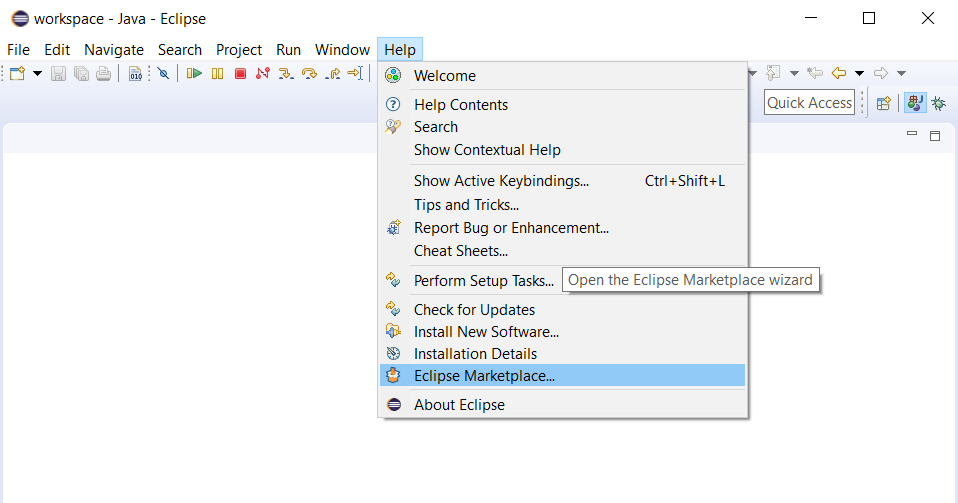
\includegraphics[width=0.8\linewidth]{images/checkstyle/Paso1.png}
    \caption{Marketplace de Eclipse}\label{}
\end{figure}

Desde el menú de ayuda de Eclipse, se accede al \textit{Marketplace}.

\begin{figure}[H]
	\centering
    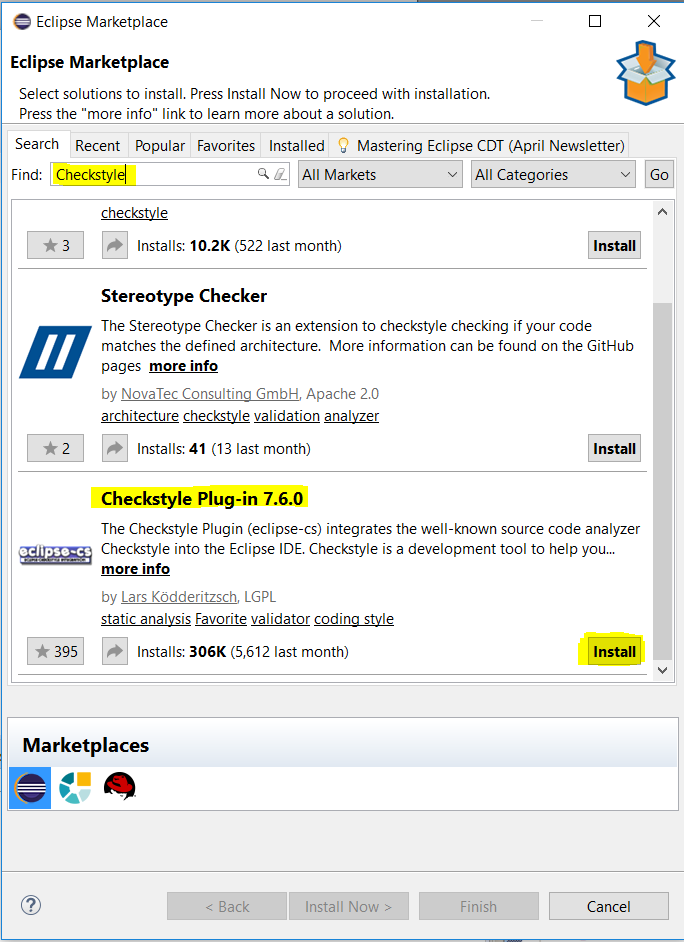
\includegraphics[width=0.6\linewidth]{images/checkstyle/Paso2.png}
    \caption{Plug-in de Checkstyle}\label{}
\end{figure}

Se busca por la herramienta \textit{Checkstyle} en la barra de búsqueda. El complemento llamado \textit{Checkstyle Plug-in 7.6.0} debería aparecer como resultado de la búsqueda. Se presiona el botón \textit{Install}.

\begin{figure}[H]
	\centering
    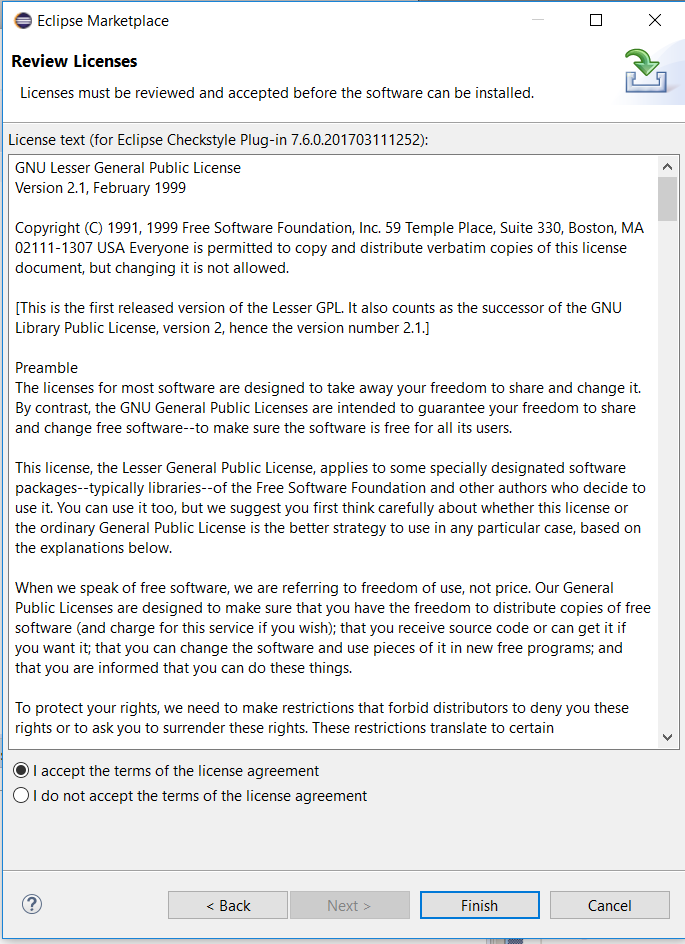
\includegraphics[width=0.6\linewidth]{images/checkstyle/Paso3.png}
    \caption{Instalación del Plug-in}\label{}
\end{figure}

Instalamos la herramienta siguiendo los pasos solicitados por el \textit{Marketplace}.

\begin{figure}[H]
	\centering
    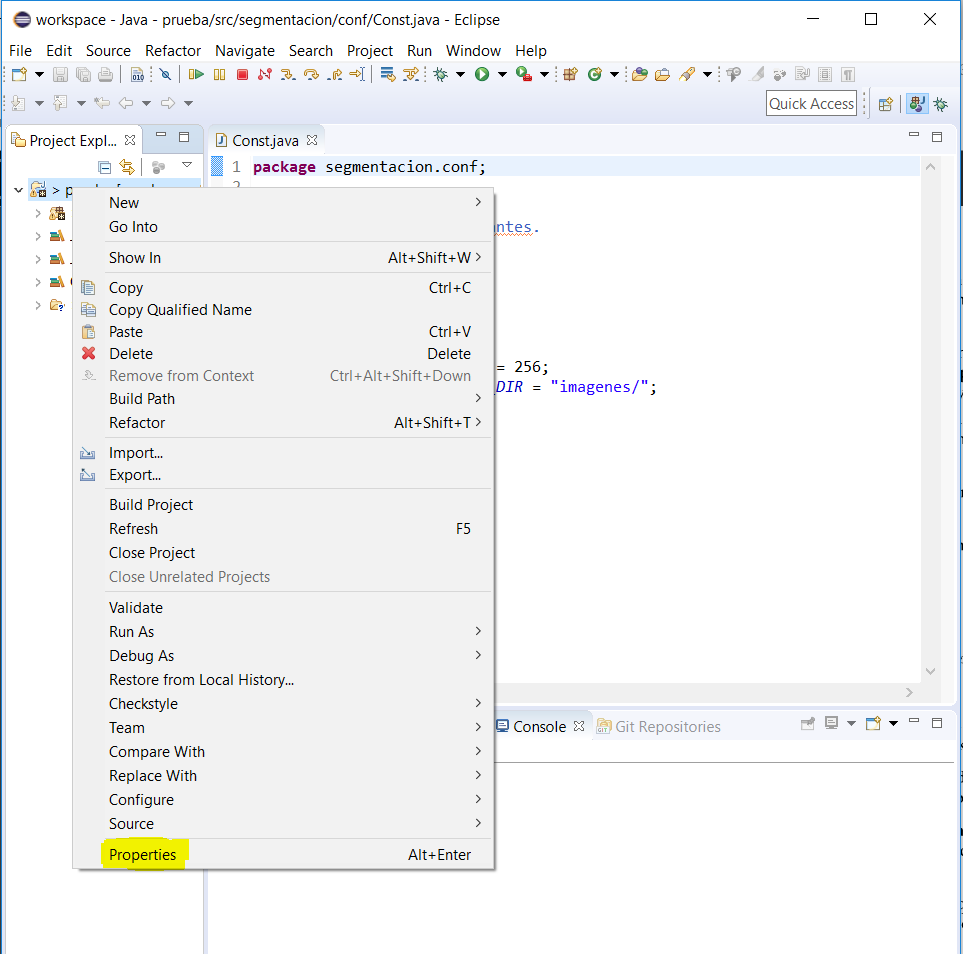
\includegraphics[width=0.6\linewidth]{images/checkstyle/Paso4.png}
    \caption{Configuración del proyecto}\label{}
\end{figure}

Una vez instalado el complemento, abrimos la ventana de propiedades del proyecto.

\begin{figure}[H]
	\centering
    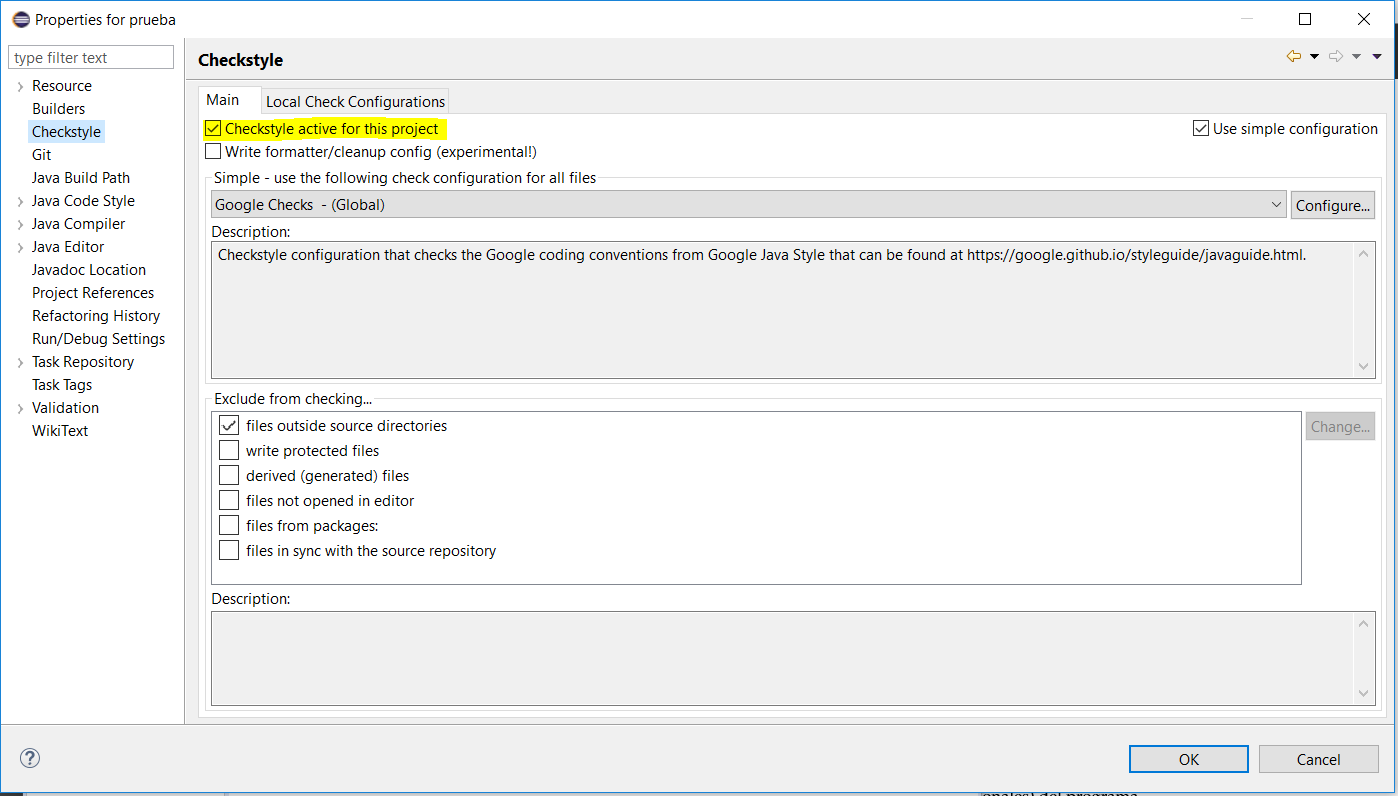
\includegraphics[width=0.8\linewidth]{images/checkstyle/Paso5.png}
    \caption{Habilitar Plug-in}
\end{figure}

Una vez en la ventana de propiedades, vamos a la pestaña \textit{Checkstyle} y marcamos la opción \textit{Checkstyle active for this project.} En esta misma pentaña podemos seleccionar el estándar de codificación(En nuestro caso, Google Java Style)



\chapter{Repositorio}

El repositorio del sistema \textit{SPACE} (github.com/jubileus95/SPACE) contiene todos los ítems de configuración del proyecto. A continuación, se muestra el procedimiento para obtener la última versión de SPACE.

\section{Obtener versión actual del sistema}

Para obtener la línea base del sistema, se puede hacer un git clone del repositorio donde esta alojado el proyecto SPACE. 

\begin{figure}[H]
	\centering
    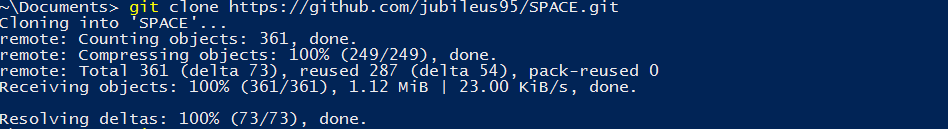
\includegraphics[width=0.8\linewidth]{images/github/repo.PNG}
    \caption{Git clone del proyecto}
\end{figure}

El URL para clonar el repositorio es el siguiente: \href{https://github.com/jubileus95/SPACE.git}{https://github.com/jubileus95/SPACE.git}

\chapter{Métricas}

Para el proyecto de SPACE, se van a emplear varias métricas para tener un mejor manejo de implementación, compreción y mantenibilidad del sotfware. Se mostraran dos métricas para los requerimientos, una para los funcionales y otra para los no funcionales.

\section{Verificación de olores de software}

Para encontrar bugs y olores de software en el código estático directamente desde el entorno de programación de Eclipse, se puede utilizar la herramienta \textit{SonarLint for Eclipse} de SonarSource (desarrolladores además de SonarQube). Para instalar la herramienta en Eclipse, se debe ir al menú \textit{Help}, seleccionar la opción \textit{Eclipse Marketplace...} y buscar \textit{SonarLint}, lo cual despliega la ventana flotante que se puede ver a continuación:

\begin{figure}[H]
	\centering
    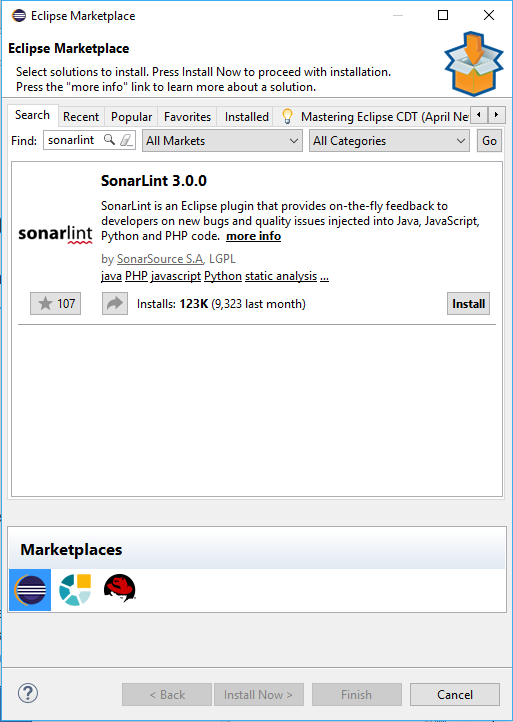
\includegraphics[width=0.5\linewidth]{images/sonarlint/1instalarSonarLint.png}
    \caption{Instalación de SonarLint}
\end{figure}

La configuración de la herramienta es automática y no requiere de intervención significativa del usuario. Para acceder a las capacidades de reportes de SonarLint, en Eclipse se debe navegar a \textit{Window $>$ Show View $>$ Other...} y una vez ahí, buscar la opción de \textit{SonarLint Report}.

\begin{figure}[H]
	\centering
    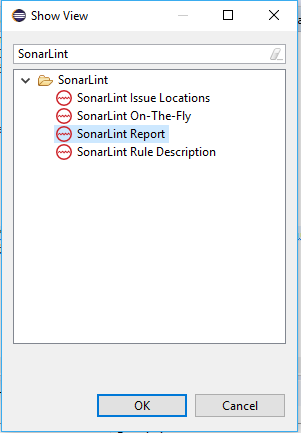
\includegraphics[width=0.5\linewidth]{images/sonarlint/2abrirVistaDeReporte.png}
    \caption{Abrir ventana de reportes de SonarLint}
\end{figure}

Para obtener un reporte completo de los bugs, olores de software y recomendaciones, basta con ejecutar el escáner sobre el proyecto, con el botón \textit{Current project}. De forma automática, se muestran los resultados del análisis, como se aprecia en la siguiente figura.

\begin{figure}[H]
	\centering
    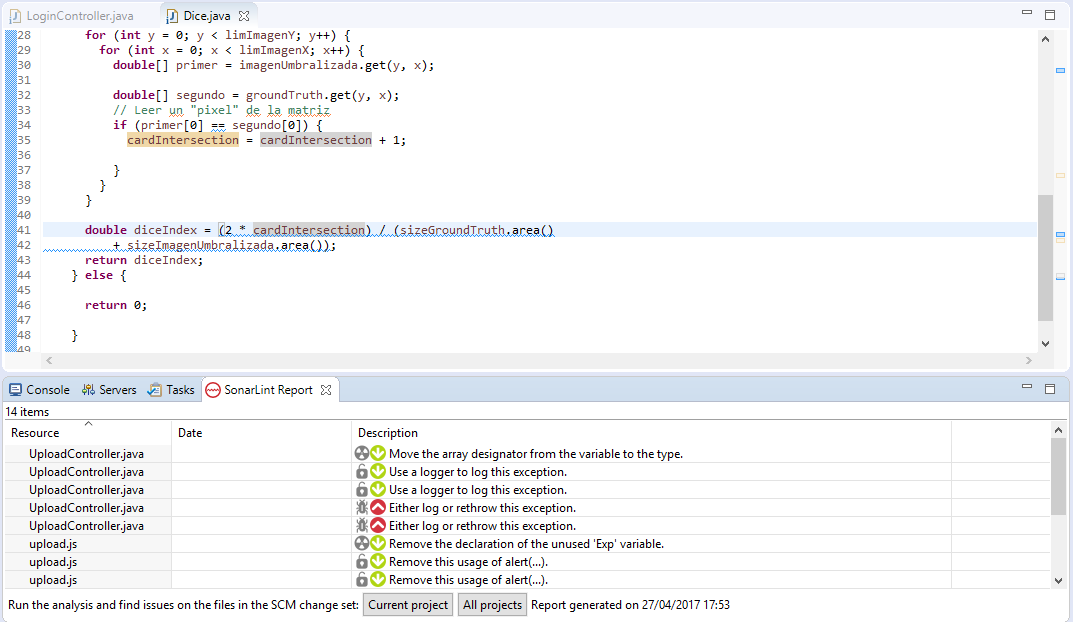
\includegraphics[width=0.9\linewidth]{images/sonarlint/3reporteDeProyecto.png}
    \caption{Reporte de SonarLint}
\end{figure}



\section{Complejidad ciclomática}

Para calcular la complejidad ciclomática en el código estático fácilmente desde el entorno de programación de Eclipse, se puede utilizar la herramienta \textit{Codecity 0.9.0}. Para instalar la herramienta en Eclipse, se debe ir al menú \textit{Help}, seleccionar la opción \textit{Eclipse Marketplace...} y buscar \textit{Codecity}, lo cual despliega la ventana flotante que se puede ver a continuación:

\begin{figure}[H]
	\centering
    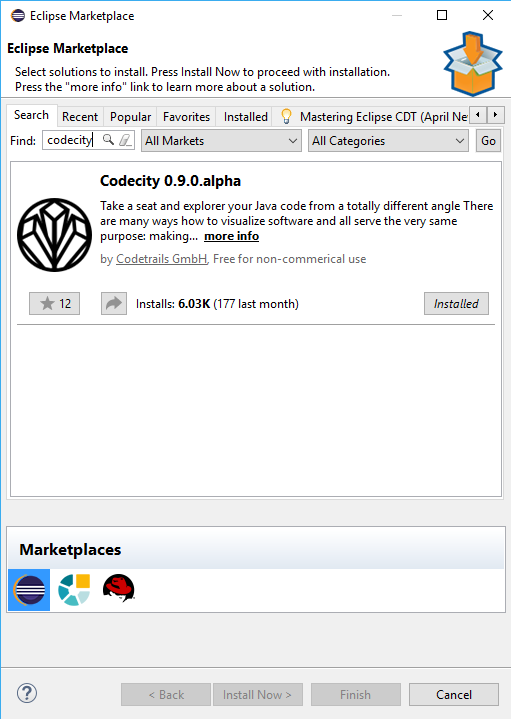
\includegraphics[width=0.8\linewidth]{images/codecity/1instalarCodecity.png}
    \caption{Instalación de Codecity}
\end{figure}

Esta herramienta tampoco requiere de más configuración para su utilización. Luego, para acceder a los  reportes de Codecity, en Eclipse se debe hacer clic derecho sobre el proyecto que se desea analizar, y de ahí seleccionar \textit{Show In $>$ Codecity}, como se muestra en la siguiente imagen.

\begin{figure}[H]
	\centering
    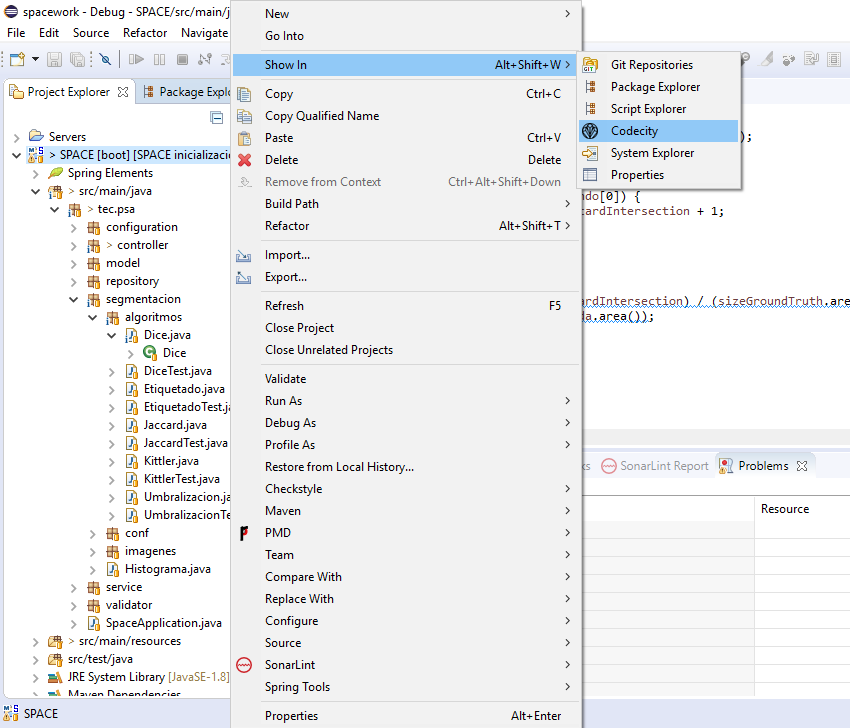
\includegraphics[width=1.0\linewidth]{images/codecity/2mostrarEnCodecity.png}
    \caption{Solicitar reporte de Codecity}
\end{figure}

Finalmente, la herramienta redirige el flujo al navegador web para visualizar diferentes métricas, entre ellas la complejidad ciclomática. Basta con seleccionar \textit{Cyclomatic complexity} como la métrica deseada. Opcionalmente, se pueden hacer ajustes sobre los colores y demás información mostrada en las dimensiones. Al pasar el puntero sobre el gráfico, la herramienta muestra más información, por ejemplo, el componente del sistema que genera el dato seleccionado en particular.

\begin{figure}[H]
	\centering
    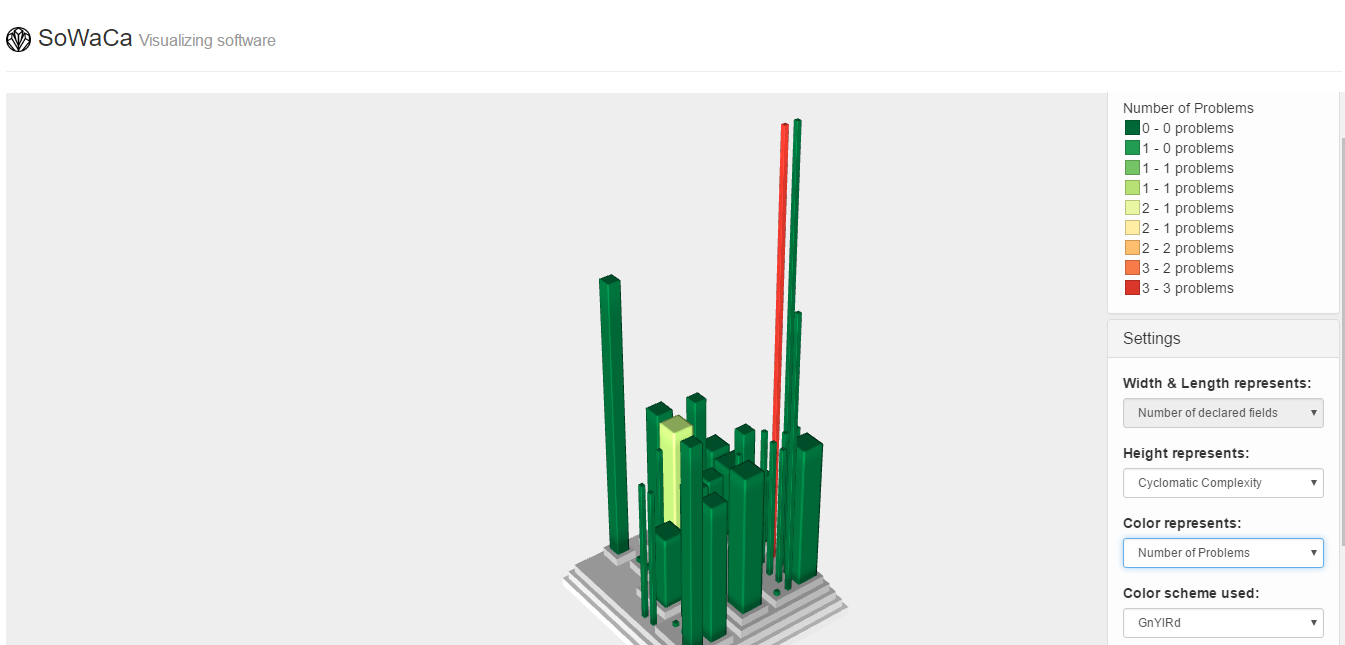
\includegraphics[width=1.0\linewidth]{images/codecity/3resultadosComplejidad.png}
    \caption{Gráfico de complejidad ciclomática en Codecity}
\end{figure}

Como puede apreciarse, existen dos barras verticales que destacan sobre las demás, que corresponden a dos archivos de código fuente del sistema que tienen una complejidad ciclomática de 6. No obstante, una complejidad ciclomática de hasta 10 es aceptable para la mantenibilidad del código.

\section{Cambios en límites de métricas}

A partir de la información adquirida anteriormente con las herramientas automáticas, se encontró que para los bugs y olores del código \textbf{(madurez)} se había definido un límite adecuado, ya que se propuso que no se dieran más de 10 olores ni más de 10 bugs en el análisis del código estático. Esto se cumplió en las métricas obtenidas.\\

Por otro lado, el límite se actualizó de un valor de 2 a 10 para la \textbf{complejidad ciclomática}, ya que se obtuvo una evaluación de 6 para un código simple. Tras hacer la investigación, se descubrió que una complejidad ciclomática de hasta 10 es aceptada como código sencillo de entender. Además, se cambió la herramienta \textit{Metrics for Eclipse} por  Los cambios sobre los límites fueron actualizados en el documento \textit{T1 - Atributos de calidad y métricas}.\\



\chapter{Especificación de pruebas unitarias}

En este apartado, se muestran la especificación de las pruebas unitarias implementadas en esta etapa del proyecto.

\section{Kittler}

\vspace{0.3cm}
\begin{center}
    \begin{tabular}{|p{4.0cm}|p{9.0cm}|}
        \hline
	    \textbf{Objetivo} & Implementación del algoritmo de Kittler determinar un valor óptimo con el fin de umbralizar una imagen. \\
        \hline
	    \textbf{Tipo de entrada} & Histograma \\
        \hline
	    \textbf{Entrada esperada} & cuadro_005.bmp \\
        \hline
	    \textbf{Entrada atípica} & Ninguna (solo imágenes) \\
        \hline
	    \textbf{Tipo de salida} & Int: \(\tau\) \(\in\) \{0, 1, 2, ... , 254, 255\} \\
        \hline
	    \textbf{Salida esperada} & 166 \\
        \hline        
    \end{tabular}
\end{center}


\section{Umbralización}

\vspace{0.3cm}
\begin{center}
    \begin{tabular}{|p{4.0cm}|p{9.0cm}|}
        \hline
	    \textbf{Objetivo} & Umbraliza una imagen en blanco y negro con un valor de umbral determinado por el algoritmo de Kittler.\\
        \hline
	    \textbf{Tipo de entrada} & Histograma, Tao (Int) \\
        \hline
	    \textbf{Entrada esperada} & cuadro_005.bmp \\
        \hline
	    \textbf{Entrada atípica} & Ninguna (solo imágenes) \\
        \hline
	    \textbf{Tipo de salida} & Mat \\
        \hline
	    \textbf{Salida esperada} & Matriz umbralizada en blanco y negro \\
        \hline        
    \end{tabular}
\end{center}


\section{Etiquetado}

\vspace{0.3cm}
\begin{center}
    \begin{tabular}{|p{4.0cm}|p{9.0cm}|}
        \hline
	    \textbf{Objetivo} & Etiqueta cada una de las células en una imagen con una característica distinguible (color). \\
        \hline
	    \textbf{Tipo de entrada} & Imagen (Mat) \\
        \hline
	    \textbf{Entrada esperada} & cuadro_005.bmp \\
        \hline
	    \textbf{Entrada atípica} & Ninguna (solo imágenes) \\
        \hline
	    \textbf{Tipo de salida} & Mat \\
        \hline
	    \textbf{Salida esperada} & Imagen etiquetada con colores secuenciales \\
        \hline        
    \end{tabular}
\end{center}


\section{Dice (nueva)}

\vspace{0.3cm}
\begin{center}
    \begin{tabular}{|p{4.0cm}|p{9.0cm}|}
        \hline
	    \textbf{Objetivo} & Calcular valor que permita medir qué tan similar es una imagen segmentada automáticamente respecto a un groundtruth. \\
        \hline
	    \textbf{Tipo de entrada} & Imagen (Mat) \\
        \hline
	    \textbf{Entrada esperada} & Dice.bmp; Dice2.bmp; Dice3.bmp; Dice4.bmp \\
        \hline
	    \textbf{Entrada atípica} & Ninguna \\
        \hline
		\textbf{Tipo de salida} & double : [0, 1] \\
        \hline
	    \textbf{Salida esperada} & 0; 0.25; 0.50; 0.75 \\
        \hline        
    \end{tabular}
\end{center}


\section{Jaccard (nueva)}
\vspace{0.3cm}
\begin{center}
    \begin{tabular}{|p{4.0cm}|p{9.0cm}|}
        \hline
	    \textbf{Objetivo} & Calcular valor que permita medir qué tan similar es una imagen segmentada automáticamente respecto a un groundtruth. \\
        \hline
	    \textbf{Tipo de entrada} & Imagen (Mat) \\
        \hline
	    \textbf{Entrada esperada} & Dice.bmp; Dice2.bmp; Dice3.bmp; Dice4.bmp \\
        \hline
	    \textbf{Entrada atípica} & Ninguna \\
        \hline
	    \textbf{Tipo de salida} & double : [0, 1] \\
        \hline
	    \textbf{Salida esperada} & 0; 0.1429; 0.3333; 0.60 \\
        \hline        
    \end{tabular}
\end{center}


\section{Subida a MongoDB (nueva)}
\vspace{0.3cm}
\begin{center}
    \begin{tabular}{|p{4.0cm}|p{9.0cm}|}
        \hline
	    \textbf{Objetivo} & Implementación de la creación e insersión de imágen de la base datos.\\
        \hline
	    \textbf{Tipo de entrada} & Image \\
        \hline
	    \textbf{Entrada esperada} & imagenr \\
        \hline
	    \textbf{Entrada atípica} & Ninguna (solo imágenes) \\
        \hline
	    \textbf{Tipo de salida} & Boolean \\
        \hline
	    \textbf{Salida esperada} & State \\
        \hline        
    \end{tabular}
\end{center}

\section{Descarga de MongoDB (nueva)}
\vspace{0.3cm}
\begin{center}
    \begin{tabular}{|p{4.0cm}|p{9.0cm}|}
        \hline
	    \textbf{Objetivo} & Implementación de la busqueda y descarga de imágen de la base datos. \\
        \hline
	    \textbf{Tipo de entrada} & String \\
        \hline
	    \textbf{Entrada esperada} & imagenr \\
        \hline
	    \textbf{Entrada atípica} & Ninguna (solo Cadenas) \\
        \hline
	    \textbf{Tipo de salida} & Image \\
        \hline
	    \textbf{Salida esperada} & imagenr (Imagen) \\
        \hline        
    \end{tabular}
\end{center}

\end{document}